\PassOptionsToPackage{svgnames}{xcolor}
\documentclass[12pt]{article}



\usepackage[margin=1in]{geometry}  
\usepackage{graphicx}             
\usepackage{amsmath}              
\usepackage{amsfonts}              
\usepackage{framed}               
\usepackage{amssymb}
\usepackage{array}
\usepackage{amsthm}
\usepackage[nottoc]{tocbibind}
\usepackage{bm}
\usepackage[object=vectorian]{pgfornament} 
\usepackage{enumitem}
\colorlet{shadecolor}{lightgray!25}
\newcommand{\sectionline}{%
  \noindent
  \begin{center}
  {\color{DarkViolet}
    \resizebox{0.5\linewidth}{1ex}
    {{%
    {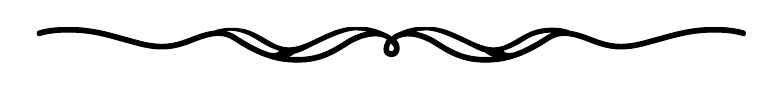
\begin{tikzpicture}
    \node  (C) at (0,0) {};
    \node (D) at (9,0) {};
    \path (C) to [ornament=85] (D);
    \end{tikzpicture}}}}}%
    \end{center}
  }

 \newcommand{\im}{\mathrm{i}}
  \newcommand{\diff}{\mathrm{d}}
  \newcommand{\be}{\mathrm{Be}}
  \newcommand{\var}{\mathrm{Var}}
  \newcommand{\expec}{\mathrm{E}}
  \newcommand{\bin}{\mathrm{Bin}}
  \newcommand{\geom}{\mathrm{Geom}}
  \newcommand{\Poi}{\mathrm{Poisson}}
  \newcommand{\nb}{\mathrm{NB}}
  \newcommand{\hg}{\mathrm{H}}
  \newcommand{\expo}{\mathrm{Exp}}
  \newcommand{\betadis}{\mathrm{Beta}}
  \newcommand{\cauchy}{\mathrm{Cauchy}}
  \newcommand{\cov}{\mathrm{cov}}
\setlength{\parindent}{0cm}
\setlength{\parskip}{0em}
\newcommand{\Lim}[1]{\raisebox{0.5ex}{\scalebox{0.8}{$\displaystyle \lim_{#1}\;$}}}
\newtheorem{definition}{Definition}[section]
\newtheorem{theorem}{Theorem}[section]
\theoremstyle{definition}
\DeclareMathOperator{\arcsec}{arcsec}
\DeclareMathOperator{\arccot}{arccot}
\DeclareMathOperator{\arccsc}{arccsc}
\setcounter{tocdepth}{1}
\begin{document}
\title{Revision notes - ST2131}
\author{Ma Hongqiang}
\maketitle
\tableofcontents

\clearpage

\section{Combinatorial Analysis}
\begin{theorem}[Generalised Basic Principle of Counting]
\hfill\\
\normalfont Suppose that $r$ experiments are to be preformed. If
\begin{itemize}
\item experiment 1 can result in $n_1$ possible outcomes;
\item experiment 2 can result in $n_2$ possible outcomes;
\item $\cdots$
\item experiment $r$ can result in $n_r$ possible outcomes;
\end{itemize}
then together there are $n_1 n_2 \cdots n_r$ possible outcomes of the $r$ experiments.
\end{theorem}
\subsection{Permutations}
\begin{theorem}[Permutation of distinct objects]
\hfill\\
\normalfont Suppose there are $n$ distinct objects, then the total number of permutations is 
\[n!\].
\end{theorem}
\begin{theorem}[General principle of permutation]
\hfill\\
\normalfont For $n$ objects of which $n_1$ are alike, $n_2$ are alike, $\ldots$, $n_r$ are alike, there are
\[
\frac{n!}{n_1!n_2!\cdots n_r!}
\]
different permutations of the $n$ objects.
\end{theorem}
\subsection{Combinations}
\begin{theorem}[General principle of combination]
\hfill\\
\normalfont If there are $n$ distinct objects, of which we choose a group of $r$ items, number of combinations equals
\[
\binom{n}{r}=\frac{n!}{r!(n-r)!}
\]
\end{theorem}
\subsubsection{Useful Combinatorial Identities}
\begin{enumerate}
\item For $1\leq r\leq n$,$\binom{n}{r}=\binom{n-1}{r-1}+\binom{n-1}{r}$
\item (\textbf{Binomial Theorem}) Let $n$ be a non-negative integer, then
\[
(x+y)^n=\sum_{k=0}^{n}\binom{n}{k}x^k y^{n-k}
\]
\item $\sum_{k=0}^{n}\binom{n}{k}=2^n$
\item $\sum_{k=0}^{n}(-1)^k\binom{n}{k}=0$
\end{enumerate}
\subsection{Multinomial Coefficients}
If $n_1+n_2+\cdots+n_r=n$, we define $\binom{n}{n_1,n_2,\cdots,n_r}$ by
\[
\binom{n}{n_1,n_2,\cdots,n_r}=\frac{n!}{n_1!n_2!\cdots n_r!}
\]
Thus $\binom{n}{n_1,n_2,\cdots,n_r}$ represents the number of possible divisions of $n$ distinct objects into $r$ distinct groups of respective sizes $n_1, n_2, \cdots, n_r$.
\begin{theorem}[Multinomial Theorem]
\[
(x_1+x_2+\cdots+x_r)^n=\sum_{(n_1,\ldots,n_r):n_1+\cdots+n_r=n}\binom{n}{n_1,n_2,\cdots,n_r}x_1^{n_1}x_2^{n_2}\cdots x_r^{n_r}
\]
\end{theorem}
\subsection{Number of Integer Solutions of Equations}
\begin{theorem}
\normalfont There are $\binom{n-1}{r-1}$ distinct \textit{positive} integer-valued vectors $(x_1,x_2,\ldots,x_r)$ that satisfies the equation
\[
x_1+x_2+\cdots+x_r=n
\]
where $x_i>0$ for $i=1,\ldots, r$
\end{theorem}
\begin{theorem}
\normalfont There are $\binom{n+r-1}{r-1}$ distinct \textit{non-negative} integer-valued vectors $(x_1,x_2,\ldots,x_r)$ that satisfies the equation
\[
x_1+x_2+\cdots+x_r=n
\]
where $x_i>0$ for $i=1,\ldots, r$
\end{theorem}
\section{Axioms of Probability}
\subsection{Sample Space and Events}
The basic objects of probability is an \textbf{experiment}: an activity or procedure that produces distinct, well-defined possibilities called \textbf{outcomes}.\\
The \textbf{sample space} is the set of all possible outcomes of an experiment, usually denoted by $S$.\\
Any subset $E$ of the sample space is an \textbf{event}.
\subsection{Axions of probability}
\textbf{Probability}, denoted by $P$, is a function on the collection of events satisfying
\begin{enumerate}[label=(\roman*)]
\item For any event $A$,
\[
0\leq P(A)\leq 1
\]
\item Let $S$ be the sample space, then
\[
P(S)=1
\]
\item For any sequence of mutually exclusive events $A_1, A_2,\ldots$(that is $A_iA_j=\varnothing$ when $i\neq j$)
\[
P\left(\cup_{i=1}^{\infty}A_i\right)=\sum_{i=1}^{\infty}P(A_i)
\]
\end{enumerate}
\subsection{Properties of Probability}
\begin{theorem}\normalfont $P(\varnothing)=0$.\end{theorem}
\begin{theorem}\normalfont For any finite sequence of mutually exclusive event $A_1,A_2,\ldots, A_n$,
\[
P\left(\cup^n_{i=1}A_i\right)=\sum^n_{i=1}P(A_i)
\]
\end{theorem}
\begin{theorem}\normalfont Let $A$ be an event, then
\[
P(A^c)=1-P(A)
\]
\end{theorem}
\begin{theorem}\normalfont If $A\subseteq B$, then
\[
P(A)+P(BA^c)=P(B)
\]
\end{theorem}
\begin{theorem}[Inclusion-exclusion Principle]\normalfont Let $A_1,A_2,\ldots,A_n$ be any events, then
\begin{equation*}
\begin{aligned}
P(A_1\cup A_2\cup \cdots\cup A_n)=&\sum_{i=1}^n P(A_i) -\sum_{1\leq i_1\leq i_2\leq n}P(A_{i_1}A_{i_2})+\cdots\\&+(-1)^{r+1}\sum_{1\leq i_1\leq\cdots\leq i_r\leq n}P(A_{i_1}\cdots A_{i_r})\\&+\cdots+(-1)^{n+1}P(A_1\cdots A_n)
\end{aligned}
\end{equation*}
\end{theorem}
\subsection{Probability as a Continuous Set Function}
\begin{definition}\normalfont A sequence of events $\{E_n\},n\geq 1$ is said to be an \textbf{increasing} sequence if
\[
E_1\subset E_2\subset \cdots \subset E_n\subset E_{n+1}\subset \cdots
\]
whereas it is said to be a \textbf{decreasing} sequence if
\[
E_1\supset E_2\supset \cdots \supset E_n\supset E_{n+1}\supset \cdots
\]
\end{definition}
\begin{definition}\normalfont If $\{E_n\},n\geq 1$ is an increasing sequence of events,\\
define new event, denoted by $\Lim{n\to\infty}E_n$ as
\[
\lim_{n\to\infty}E_n=\cup^{\infty}_{i=1}E_i
\]
Similarly, if $\{E_n\},n\geq 1$ is an decreasing sequence of events, define new event, denoted by $\Lim{n\to\infty}E_n$ as
\[
\lim_{n\to\infty}E_n=\cap^{\infty}_{i=1}E_i
\]
\end{definition}
\begin{theorem}\normalfont If $\{E_n\},n\geq 1$ is either an increasing or a decreasing sequence of events, then
\[
\lim_{n\to\infty}P(E_n)=P\left(\lim_{n\to\infty}E_n\right)
\]
\end{theorem}
\clearpage
\section{Conditional Probability and Independence}
\subsection{conditional Probabilities}
\begin{definition}\normalfont Let $A$ and $B$ be two events. Suppose that $P(A)>0$, the \textbf{conditional probability} of $B$ given $A$ is defined as
\[
\frac{P(AB)}{P(A)}
\]
and is denoted by $P(B|A)$.\\
Suppose $P(A)>0$, then $P(AB)=P(A)P(B|A)$.
\end{definition}
\begin{theorem}[General Multiplication Rule]
\hfill\\\normalfont Let $A_1,A_2,\ldots,A_n$ be $n$ events, then
\[
P(A_1A_2\cdots A_n)=P(A_1)P(A_2|A_1)P(A_3|A_1A_2)\cdots P(A_n|A_1A_2\cdots A_{n-1})
\]
\end{theorem}
\subsection{Bayes' Formulas}
Let $A$ and $B$ be any two events, then
\[
P(B)=P(B|A)P(A)+P(B|A^c)P(A^c)
\]
\begin{definition}\normalfont We say that $A_1,A_2,\ldots,A_n$ \textbf{partitions} the sample space $S$ if:
\begin{itemize}
\item They are \textbf{mutually exclusive}, meaning $A_i\cap A_j = \varnothing\;\forall i\neq j$.
\item THey are collectively exclusive, meaning $\cup_{i=1}^{n}A_i=S$
\end{itemize}
\end{definition}
\begin{theorem}[Bayes' First Formula]
\hfill\\\normalfont Suppose the events $A_1,A_2,\ldots,A_n$ partitions the sample space. Assume further that $P(A_i)>0$ for $1\leq i\leq n$. Let $B$ be any event, then
\[
P(B)=P(B|A_1)P(A_1)+\cdots+P(B|A_n)P(A_n)
\]
\end{theorem}
\begin{theorem}[Bayes' Second Formula]
\hfill\\\normalfont Suppose the events $A_1,A_2,\ldots,A_n$ partitions the sample space. Assume further that $P(A_i)>0$ for $1\leq i\leq n$. Let $B$ be any event, then for any $1\leq i \leq n$,
\[
P(A_i|B)=\frac{P(B|A_i)P(A_i)}{P(B|A_1)P(A_1)+\cdots+P(B|A_n)P(A_n)}
\]
\end{theorem}
\subsection{Independent Events}
\begin{definition}\normalfont Two events $A$ and $B$ are said to be \textbf{independent} if
\[
P(AB)=P(A)P(B)
\]
They are said to be dependent otherwise.
\end{definition}
\begin{theorem}\normalfont If $A$ and $B$ are independent, then so are
\begin{enumerate}
\item $A$ and $B^c$
\item $A^c$ and $B$
\item $A^c$ and $B^c$
\end{enumerate}
\end{theorem}
\begin{definition}\normalfont Events $A_1,A_2,\ldots, A_n$ are said to be \textbf{independent}, if for eveery subcollection of events $A_{i_1},\ldots,A_{i_r}$, we have
\[
P(A_{i_1}\cdots A_{i_r}) =P(A_{i_1})P(A_{i_r}) 
\] 
\end{definition}
\subsection{$P(\cdot|A)$ is a Probability}
\begin{theorem}\normalfont Let $A$ be an event with $P(A)>0$. Then the following three conditions hold.
\begin{enumerate}
\item For any event $B$, we have
\[
0\leq P(B|A)\leq 1
\]
\item 
\[
P(S|A)=1
\]
\item Let $B_1.B_2,\ldots$ be a sequence of mutually exclusive events, then
\[
P(\cup_{k=1}^{\infty}B_k|A)=\sum_{k=1}^\infty P(B_k|A)
\]
\end{enumerate}
\end{theorem}
\clearpage
\section{Random Variables}
\subsection{Random Variables}
\begin{definition}\normalfont A \textbf{random variable} $X$, is a mapping from the sample space to real numbers.
\end{definition}
\subsection{Discrete Random Variables}
\begin{definition}\normalfont A random variable is said to be \textbf{discrete} if the range of $X$ is either finite or countably infinite.
\end{definition}
\begin{definition}\normalfont Suppose that random variable $X$ is discrete, taking values $x_1,x_2\ldots$, then the \textbf{probability mass function} of $X$, denoted by $p_X$, is defined as
\begin{equation*}
p_X(x)=\begin{cases}
P(X=x)&\text{if }x=x_1,x_2,\ldots\\
0&\text{otherwise}
\end{cases}
\end{equation*}
\end{definition}
Properties of the probability mass function include
\begin{enumerate}
\item $p_X(x_i)\geq 0$ for $i=1,2,\ldots$;
\item $p_X(x)=0$ for other values of $x$;
\item Since $X$ must take on one of the values of $x_i$, $\sum_{i=1}^\infty p_X(x_i)=1$.
\end{enumerate}
\begin{definition}\normalfont The \textbf{cumulative distribution function} of $X$, is defined as
\[
F_X:\mathbb{R}\to\mathbb{R}
\] 
where
\[
F_X(x)=P(X\leq x)\;\forall x\in\mathbb{R}
\]
\end{definition}
\textbf{Remark}: SUppose that $X$ is discrete and takes values $x_1,x_2,\ldots$ where $x_1<x_2<x_3<\cdots$. Note then that $F$ is a step function, that is, $F$ is constant in the interval $[x_{i-1},x_i)$ ($F$ takes value $p(x_1)+\cdots+p(x_{i-1})$), and then take a jump of size = $p(x_i)$.
\subsection{Expected Value}
\begin{definition}\normalfont If $X$ is a discrete random variable having a probability mass function $p_X$, the \textbf{expectation} or \textbf{expected value} of $X$, denoted by $\expec(X)$ or $\mu_X$ is defined by
\[
\expec(X)=\sum_{x}xp_X(x)
\]
\end{definition}
\begin{definition}[Bernoulli Random Variable]
\hfill\\\normalfont Suppose $X$ takes only two values $0$ and $1$ with
\[
P(X=0)=1-p\;\;\;\;\;\text{and}\;\;\;\;\;P(X=1)=p
\]
We call this random variable a \textbf{Bernoulli} random variable of parameter $p$. And we denote it by $X\sim\be(p)$.
\end{definition}
\subsection{Expectation of a Function of a Random Variable}
\begin{theorem}\normalfont If $X$ is a discrete random variable that takes values $x_i$, $i\geq 1$, with respective probabilities $p_X(x_i)$, then for any real value function $g$
\[
\begin{aligned}
\expec[g(x)]&=\sum_i g(x_i)p_X(x_i)\;\;\;\text{or equivalently}\\
&=\sum_x g(x)p_X(x)
\end{aligned}
\]
\end{theorem}
\begin{theorem}\normalfont Let $a$ and $b$ be constants, then
\[
\expec[aX+b]=a\expec(X)+b
\]
\end{theorem}
\begin{theorem}[Tail Sum Formula for Expectation]
\hfill\\\normalfont For \textit{nonnegative integer-valued} random variable $X$,
\[
\expec(X)=\sum_{k=1}^\infty P(X\geq k)=\sum_{k=0}^\infty P(X>k)
\]
\end{theorem}
\subsection{Variance and Standard Deviation}
\begin{definition}\normalfont If $X$ is a random variable with mean $\mu$, then the \textbf{variance} of $X$, denoted by $\var(X)$, is defined by
\[
\var(X)=\expec(X-\mu)^2
\]
\end{definition} 
An alternative formula for variance is:
\[
\var(X)=\expec(X^2)-[\expec(X)]^2
\]
\textbf{Remark}:
\begin{enumerate}
\item $\var(X)\geq 0$
\item $\var(X)=0$ if and only if $X$ is a degenerate random variable
\item $\expec(X^2)\geq [\expec(X)]^2\geq 0$
\item $\var(aX+b)=a^2\var(X)$
\end{enumerate}
\subsection{Discrete Random Variable arising from Repeated Trials}
\begin{enumerate}
\item \textbf{Bernoulli random variable}, denoted by $\be(p)$.\\
We only perform the Bernoulli Trial once and define
\[
X=\begin{cases}
1\;\;\;\;\;&\text{if it is a success}\\
0\;\;\;\;\;&\text{if it is a failure}
\end{cases}
\]
Here,
\[
P(X=1)=p, P(X=0)=1-p
\]
and
\[
\expec(X)=p,\;\;\;\var(X)=p(1-p)
\]
\item \textbf{Binomial random variable},denoted by $\bin(n,p)$\\
We perform the experiment (under identical conditions and independently) $n$ times and define
\[
X = \text{number of successes in }n \text{ Bernoulli}(p)\text{ trials}
\]
Therefore, $X$ takes values $0,1,\ldots,n$. In fact, for $0\leq k\leq n$,
\[
P(X=k)=\binom{n}{k} p^kq^{n-k}
\]
Here,
\[
\expec(X)=np, \;\;\;\;\;\var(X)=np(1-p)
\]
Also, a useful fact is
\[
\frac{P(X=k+1)}{P(X=k)}=\frac{p}{1-p}\frac{n-k}{k+1}
\]
\item \textbf{Geometric random variable}, denoted by $\geom(p)$\\
Define the random variable
\[
X=\text{number of Bernoulli}(p) \text{ trials required to obtain the first success}
\]
Here $X$ takes values $1,2,3,\ldots$ and so on. In fact, for $k\geq 1$,
\[
P(X=k)=pq^{k-1}
\]
And,
\[
\expec(X)=\frac{1}{p}\;\;\;\;\;\var(X)=\frac{1-p}{p^2}
\]
\item \textbf{Negative Binomial random variable}, denoted by $\nb{r,p}$\\
Define the random variable
\[
X=\text{number of Bernoulli}(p)\text{ trials required to obtain }r\text{ success.}
\]
Here, $X$ takes values $r,r+1,\ldots$ and so on. In fact, for $k\geq r$,
\[
P(X=k)=\binom{k-1}{r-1}p^rq^{k-r}
\]
And
\[
\expec(X)=\frac{r}{p}\;\;\;\;\;\var(X)=\frac{r(1-p)}{p^2}
\]
\end{enumerate}
\subsection{Poisson Random Variable}
A random variable $X$ is said to have a \textbf{Poisson} distribution with parameter $\lambda$ if $X$ takes values $0,1,2\ldots$ with probabilities given as:
\[
P(X=k) = \frac{e^{-\lambda}\lambda^k}{k!}
\]
And
\[
\expec(X)=\lambda\;\;\;\;\;\var(X)=\lambda
\]
Poisson distribution of parameter $\lambda:=np$ can be used as an approximation for a binomial distribution with parameter $(n,p)$, when $n$ is large and $p$ is small such that $np$ is moderate.\\
(\textbf{Poisson Paradigm}) Consider $n$ events, with $p_i$ equal to the probability that event $i$ occurs, $i = 1,\ldots, n$. If all the $p_i$ are small and trials are either independent or at most weakly dependent, then the number of these events that occur approximately has a Poisson distribution with mean $\sum_{i=1}^n p_i :=\lambda$.
Another use is Poisson process.
\subsection{Hypergeometric Random Variable}
Suppose that we have a set of $N$ balls, of which $m$ are red and $N-m$ is blue. We choose $n$ of these balls, \textit{without replacement}, and define $X$ to be the number of red balls in our sample. Then
\[
P(X=x)=\frac{\binom{m}{x}\binom{N-m}{n-x}}{\binom{N}{n}}
\]
for $x = 0,1,\ldots,N$.
A random variable whose probability mass function is given as the above equation for some values of $n,N,m$ is said to be a \textbf{hypergeometric} random variable. and is denoted by $\hg(n,N,m)$. Here,
\[
\expec(X)=\frac{nm}{N},\;\;\;\;\;\var(X)=\frac{nm}{N}\left[\frac{(n-1)(m-1)}{(N-1)}+1-\frac{nm}{N}\right]
\]
\subsection{Expected Value of Sums of Random Variables}
\begin{theorem}
\[
\expec[X]=\sum_{s\in S}X(s)p(s)
\]
\end{theorem}
\begin{theorem}
\normalfont
For random variables $X_1,X_2,\ldots, X_n$,
\[
\expec\left[\sum_{i=1}^n X_i\right]=\sum_{i=1}^n \expec[X_i]
\]
\end{theorem}
\subsection{Distribution Functions and Probability Mass Function}
\subsubsection{Properties of distribution function}
\begin{enumerate}
\item $F_X$ is a nondecreasing function.
\item $\Lim{b\to\infty}F_X(b)=1$
\item $\Lim{b\to-\infty}F_X(b)=0$
\item $F_X$ is right continuous. That is for any $b\in\mathbb{R}$
\[
\lim_{x\to b^+}F_X(x)=F_X(b)
\]
\end{enumerate}
\subsubsection{Useful Calculations}
\begin{enumerate}
\item Calculating probabilities from density function
\begin{enumerate}
\item $P(a<X\leq b)=F_X(b)-F_X(a)$
\item $P(X<b)=\Lim{n\to\infty}F(b-\frac{1}{n})$
\item $P(X=a)=F_X(a)-F_X(a^-)$ where $F_X(a^-)=\Lim{x\to a^-}F_X(x)$
\end{enumerate}
\item Calculating probabilities from probability mass function
\[
P(A)=\sum_{x\in A}p_X(x)
\]
\item Calculate probability mass function from density function
\[
p_X(x)=F_X(x)-F_X(x^-)
\]
\item Calculate density function from probability mass function
\[
F_X(x)=\sum_{y\leq x}p_X(y)
\]
\end{enumerate}
\clearpage
\section{Continuous Random Variable}
\subsection{Introduction}
\begin{definition}\normalfont We say that $X$ is a \textbf{continuous} random variable if there exists a non-negative function $f_X$, defined for all real $x\in\mathbb{R}$, having the property that, for any set $B$ of real numbers,
\[
P(X\in B)=\int_B f_X(x)\diff x
\]
The function $f_X$ is called the \textbf{probability density function} of the random variable $X$.\\
For instance, letting $B = [a,b]$, we have
\[
P(a\leq X\leq b) = \int_a^b f_X(x)\diff x
\]
\end{definition}
\begin{definition}\normalfont We defined the \textbf{distribution function} of $X$ by
\[
F_X(x)=P(X\leq x) = \int_{-\infty}^x f_X(x)\diff x
\]
and using the Fundamental Theorem of Calculus,
\[
F_X^\prime (x)=f_X(x)
\]
\end{definition}
\begin{theorem}[Properties of Distribution Function]
\begin{enumerate}
\item $P(X=x)=0\forall x\in\mathbb{R}$.
\item $F_X$ is continuous.
\item For any $a,b\in\mathbb{R}$, where $a<b$,
\[
P(a\leq X\leq b) = P(a<X\leq b)=P(a\leq X<b)=P(a<X<b)
\]
\end{enumerate}
\end{theorem}
\subsection{Expectation and Variance of Continuous Random Variables}
\begin{definition}\normalfont Let $X$ be a continuous random variable with probability density function $f_X$, then
\[
\begin{aligned}
\expec(X)&=\int_{-\infty}^\infty xf_X(x)\diff x\\
\var(X)&=\int_{-\infty}^\infty (x^2-\expec(X)^2)f_X(x)\diff x
\end{aligned}
\]
\end{definition}
\begin{theorem}\normalfont If $X$ is a continuous random variable with probability density function $f_X$, then for any real value function $g$
\begin{enumerate}
\item 
\[
\expec[g(x)]=\int_{-\infty}^\infty g(x)f_X(x)\diff x
\]
\item Same linearity Property:
\[
\expec(aX+b)=a\expec(X)+b
\]
\item Same alternative formula for variance
\[
\var(X)=\expec(X^2)-[\expec(X)]^2
\]
\end{enumerate}
\end{theorem}
\begin{theorem}[Tail sum formula]
\hfill\\\normalfont Suppose $X$ is a nonnegative continuous random variable, then
\[
\expec(X)=\int_0^\infty P(X>x)\diff x =\int_0^\infty P(X\geq x)\diff x
\]
\end{theorem}
\begin{theorem}\normalfont We have $\var(aX+b)=a^2\var(X)$.
\end{theorem}
\subsection{Uniform distribution}
A random variable $X$ is said to be \textbf{uniformly} distributed over the interval $(a,b)$ if its probability density function is given by
\[
f_X(x)=\begin{cases}
1,&0<x<1\\
0, &\text{otherwise}
\end{cases}
\]
We denote this by $X\sim U(0,1)$.\\
Finding $F_X$:
\[
F_X(x) = \int_{-\infty}^xf_X(y)\diff y=\begin{cases}
0,&\text{if }x<0\\
x,&\text{if }0\leq x<1\\
1,&\text{if }1\leq x
\end{cases}
\]
In general, for $a<b$, a random variable $X$ is uniformly distributed over the interval $(a,b)$ if its probability density function is given by
\[
f_X(x)=\begin{cases}
\frac{1}{b-a},&a<x<b\\
0, &\text{otherwise}
\end{cases}
\]
We denote this by $X\sim U(a,b)$.
In a similar way,
\[
F_X(x)=\int_{-\infty}^xf_X(y)\diff y = \begin{cases}
0,&\text{if }x<a\\
\frac{x-a}{b-a},&\text{if }a\leq x<b\\
1,&\text{if }b\leq x
\end{cases}
\]
It was shown that
\[
\expec(X)=\frac{a+b}{2}\;\;\;\;\;\var(X)=\frac{(b-a)^2}{12}
\]
\subsection{Normal Distribution}
A random variable is said to be \textbf{normally} distributed with parameters $\mu$ and $\sigma^2$ if its probability density function is given by
\[
f_X(x)=\frac{1}{\sqrt{2\pi}\sigma}e^{-\frac{1}{2\sigma^2}(x-\mu)^2}
\]
We denote this by $X\sim N(\mu, \sigma^2)$.
The density function is \textbf{bell-shaped}, always positive, symmetric at $\mu$ and attains its maximum at $x=\mu$.\\
A normal random variable is called a \textbf{standard normal} random variable when $\mu=0$ and $\sigma=1$ and is denoted by $Z\sim N(0,1)$. Its probability density function is denoted by $\phi$ and its distribution function by $\Phi$. 
\[
\begin{aligned}
\phi(x)&=\frac{1}{\sqrt{2\pi}}e^{-\frac{1}{2}x^2}\\
\Phi(x)&=\frac{1}{\sqrt{2\pi}}\int_{-\infty}^x e^{-\frac{1}{2}y^2}\diff y
\end{aligned}
\]
An observation: Let $Y\sim N(\mu,\sigma^2)$ and $Z\sim N(0,1)$, then
\[
P(a<Y\leq b) =P\left(\frac{a-\mu}{\sigma}<Z<\frac{b-\mu}{\sigma}\right) = \Phi\left(\frac{b-\mu}{\sigma}\right)-Phi\left(\frac{a-\mu}{\sigma}\right)
\]
\begin{theorem}[Properties of Standard Normal]
\begin{enumerate}
\item $P(Z\geq 0) = P(Z\leq 0) = 0.5$.
\item $-Z\sim N(0,1)$
\item $P(Z\leq x) = 1-P(Z>x)$
\item $P(Z\leq -x) = P(Z\geq x)$
\item If $Y\sim N(\mu, \sigma^2)$, then $X=\frac{Y-\mu}{\sigma}\sim N(0,1)$
\item If $X\sim N(0,1)$, then $Y=aX+b\sim N(b,a^2)$
\end{enumerate}
\end{theorem}
Important facts:
\begin{enumerate}
\item If $Y\sim N(\mu,\sigma^2)$, then $\expec(Y)=\mu$ and $\var(Y)=\sigma^2$.
\item If $Z\sim N(0,1)$, then $\expec(Z)=0$ and $\var(Z)=1$.
\end{enumerate}
\begin{definition}\normalfont The $q$th quantile of a random variable $X$ is defined as a number $z_q$ so that $P(X\leq z_q) = q$.
\end{definition}
\subsection{Exponential Distribution}
A random variable $X$ is said to be \textbf{exponentially} distributed with parameter $\lambda>0$ if its probability density function is given by
\[
f_X(x) = \begin{cases}
\lambda e^{-\lambda x}&\text{if }x\geq 0\\
0&\text{if }x<0
\end{cases}
\]
The distribution function of $X$ is given by
\[
F_X(x)=\begin{cases}
0&x\leq 0\\
1-e^{-\lambda x}&x>0
\end{cases}
\]
Exponential distribution has memoryless property.
\[
P(X>s+t\mid X>s)=P(X>t)
\]
Mean and variance of $X\sim\expo(\lambda)$:
\[
\expec(X)=\frac{1}{\lambda}\;\;\;\;\;\var(X)=\frac{1}{\lambda^2}
\]
\subsection{Gamma Distribution}
A random variable $X$ is said to have a \textbf{gamma distribution} with parameters $(\alpha, \lambda)$, denoted by $X\sim\Gamma(\alpha, \lambda)$, if its probability density function is given by
\[
f_X(x)=\begin{cases}
\frac{\lambda^\alpha}{\Gamma(\alpha)}e^{-\lambda x}x^{\alpha-1},&x\geq 0\\
0&x<0
\end{cases}
\]
where $\lambda>0$, $\alpha>0$, and $\Gamma(\alpha)$, called the \textbf{gamma function}, is defined by
\[
\Gamma(\alpha) = \int_0^\infty e^{-y}y^{\alpha-1}\diff y
\]
\textbf{Remark}:
\begin{enumerate}
\item $\Gamma(1)=1$.
\item $\Gamma(\alpha) =(\alpha-1)\Gamma(\alpha-1)$
\item For integral values of $\alpha = n$, $\Gamma(n)=(n-1)!$.
\item $\Gamma(1,\lambda)=\expo(\lambda)$.
\item $\Gamma(\frac{1}{2})=\sqrt{\pi}$
\end{enumerate}
\subsection{Beta Distribution}
A random variable $X$ is said to have a \textbf{beta distribution} with parameter $(a,b)$, denoted by $X\sim \betadis(a,b)$, if its density is given by
\[
f(x)=\begin{cases}
\frac{1}{B(a,b)}x^{a-1}(1-x)^{b-1}&0<x<1\\
0&\text{otherwise}
\end{cases}
\]
where
\[
B(a,b)=\int_0^1x^{a-1}(1-x)^{b-1}\diff x
\]
is known as the \textbf{beta function}.\\
It can be shown that
\[
B(a,b)=\frac{\Gamma(a)\Gamma(b)}{\Gamma(a+b)}
\]
If $X\sim\beta(a,b)$, then
\[
\expec[X]=\frac{a}{a+b}\;\;\;\text{and}\;\;\;\var(X)=\frac{ab}{(a+b)^2(a+b+1)}
\]
\subsection{Cauchy Distribution}
A random variable $X$ is said to have a \textbf{Cauchy distribution} with parameter $\theta$, $-\infty<\theta<\infty$, denoted by $X\sim\cauchy(\theta)$, if its density is given by
\[
f(x)=\frac{1}{\pi}\frac{1}{1+(x-\theta)^2},\;\;\;-\infty<x<\infty 
\]
\subsection{Approximation of Binomial Random Variables}
\begin{theorem}[De Moivre-Laplace Limit Theorem]
\hfill\\\normalfont Suppose that $X\sim \bin(n,p)$. Then for any $a<b$
\[
P\left(a\leq\frac{X-np}{\sqrt{npq}}\leq b\right)\to\Phi(b)-\Phi(a)
\]
as $n\to\infty$, where $q=1-p$.\\
That is,
\[
\bin(n,p)\approx N(np,npq)
\]
Equivalently,
\[
\frac{X-np}{\sqrt{npq}}\approx Z
\]
where $Z\sim N(0,1)$.
\textbf{Remark}: The normal approximation will be generally quite good for values of $n$ satisfying $np(1-p)\geq 10$.\\
Approximation is further improved if we incorporate \textbf{continuity correction}.\\
If $X\sim \bin(n,p)$, then
\[
\begin{aligned}
P(X=k)&=P\left(k-\frac{1}{2}\leq X\leq k+\frac{1}{2}\right)\\
P(X\geq k)&=P\left(X\geq k-\frac{1}{2}\right)\\
P(X\leq k)&=P\left(X\leq k+\frac{1}{2}\right)
\end{aligned}
\]
\end{theorem}
\subsection{Distribution of a Function of a Random Variable}
\begin{theorem}\normalfont Let $X$ be a continuous random variable having probability density function $f_X$. Suppose that $g(x)$ is a strictly monotonic(increasing or decreasing), differentiable (and thus continuous) function of $x$. Then the random variable $Y$ defined by $Y=g(x)$ has a probability density function given by
\[
f_Y(y)=\begin{cases}
f_X(g^{-1}(y))|\frac{\diff}{\diff y}g^{-1}(y)|,&\text{if }y=g(x)\text{ for some }x\\
0,&\text{if }y\neq g(x)\text{ for all }x
\end{cases}
\]
\end{theorem}
\clearpage
\section{Jointly Distributed Random Variables}
\subsection{Joint Distribution Functions}
\begin{definition}\normalfont For any two random variables $X$ and $Y$ defined on the same sample space, we defined the \textbf{joint distribution function of }$X$ and $Y$ by
\[
F_{X,Y}(x,y)=P(X\leq x,Y\leq y)\;\;\;\text{for} x,y\in\mathbb{R}
\]
The distribution function of $X$ can be obtained from the joint density function of $X$ and $Y$ in the following way:
\[
F_X(x)=\Lim{y\to\infty}F_{X,Y}(x,y)
\]
We call $F_X$ the \textbf{marginal distribution function} of $X$.\\
Similarly,
\[
F_Y(y)=\Lim{x\to\infty}F_{X,Y}(x,y)
\]
and $F_Y$ is called the \textbf{marginal distribution function} of $Y$.
\end{definition}
\begin{theorem}[Some Useful Calculations]
\hfill\\\normalfont
Let $a,b,a_1\leq a_2, b_1\leq b_2$ be real numbers, then
\[
P(X>a, Y>b) = 1-F_X(a)-F_Y(b)+F_{X,Y}(a,b)
\]
\[
P(a_1<X\leq a_2, b_1<Y\leq b_2)=F_{X,Y}(a_2,b_2)-F_{X,Y}(a_1,b_2)+F_{X,Y}(a_1,b_1)-F_{X,Y}(a_2,b_1)
\]
\end{theorem}
\subsubsection{Jointly Discrete Random Variables}
In the case when both $X$ and $Y$ are discrete random variables, we define the \textbf{joint probability mass function of }$X$ and $Y$ as:
\[
p_{X,Y}(x,y)=P(X=x,Y=y)
\]
We can recover the probability mass function of $X$ and $Y$ in the following manner:
\[
p_X(x)=P(X=x)=\sum_{y\in\mathbb{R}}p_{X,Y}(x,y)
\]
\[
p_Y(y)=P(Y=y)=\sum_{x\in\mathbb{R}}p_{X,Y}(x,y)
\]
We call $p_X$ the \textbf{marginal probability mass function} of $X$ and $p_Y$ the \textbf{marginal probability mass function} of $Y$.
\begin{theorem}[Some useful formulas]
\hfill\\\normalfont
\begin{enumerate}
\item
\[
P(a_1<X\leq a_2,b_1<Y\leq b_2) = \sum_{a_1<X\leq a_2}\sum_{b_1<Y\leq b_2}p_{X,Y}(x,y)
\]
\item
\[
F_{X,Y}(a,b) = P(X\leq a, Y\leq b)=\sum_{X\leq a}\sum_{Y\leq b}p_{X,Y}(x,y)
\]
\item
\[
P(X>a, Y>b) = \sum_{X> a}\sum_{Y> b}p_{X,Y}(x,y)
\]
\end{enumerate}
\end{theorem}
\subsubsection{Jointly Continuous Random Variables}
We say that $X$ and $Y$ are \textbf{jointly continuous random variables} if there exists a function (which is denoted by $f_{X,Y}$, called the \textbf{jointly probability density function} of $X$ and $Y$) if for every set $C\subset \mathbb{R}^2$, we have
\[
P((X,Y)\in C)=\iint_{(x,y)\in C}f_{X,Y}(x,y)\diff x\diff y
\]
\begin{theorem}[Some useful formulas]
\begin{enumerate}
\item Let $A,B\subset\mathbb{R}^2$, take $C=A\times B$ above
\[
P(X\in A, Y\in B) = \int_A\int_Bf_{X,Y}(x,y)\diff y\diff x
\]
\item In particular, let $a_1,a_2,b_1,b_2\in\mathbb{R}$ where $a_1<a_2$ and $b_1<b_2$, we have
\[
P(a_1<X\leq a_2, b_1<Y\leq b_2) = \int_{a_1}^{a_2}\int_{b_1}^{b_2}f_{X,Y}(x,y)\diff y\diff x
\]
\item Let $a,b\in\mathbb{R}$, we have
\[
F_{X,Y}(a,b) = P(X\leq a, Y\leq b) = \int_{-\infty}^a\int_{-\infty}^{b}f_{X,Y}(x,y)\diff y \diff x
\]
As a result of this,
\[
f_{X,Y}(x,y) = \frac{\partial^2}{\partial x\partial y}F_{X,Y}(x,y)
\]
\end{enumerate}
\end{theorem}
\begin{definition}\normalfont The marginal probability density function of $X$ is given by
\[
f_X(x)=\int_{-\infty}^\infty f_{X,Y}(x,y)\diff y
\]
Similarly, the marginal probability density function of $Y$ is given by
\[
f_Y(y)=\int_{-\infty}^\infty f_{X,Y}(x,y)\diff x
\]
\end{definition}
\subsection{Independent Random Variables}
Two random variables $X$ and $Y$ are said to be \textbf{independent} if
\[
P(X\in A, Y\in B) = P(X\in A)P(Y\in B)\;\;\;\text{for any }A,B\subset \mathbb{R}
\]
\begin{theorem}[For jointly discrete random variables]
\hfill\\\normalfont The following three statements are equivalent:
\begin{enumerate}
\item Random variables $X$ and $Y$ are indepedent.
\item For all $x,y\in\mathbb{R}$, we have
\[
f_{X,Y}(x,y)=f_X(x)f_Y(y)
\]
\item For all $x,y\in\mathbb{R}$, we have
\[
F_{X,Y}(x,y)=F_X(x)F_Y(y)
\]
\end{enumerate}
\end{theorem}
\begin{theorem}\normalfont Random variables $X$ and $Y$ are independent if and only if there exist functions $g,h:\mathbb{R}\to\mathbb{R}$ such that for all $x,y\in\mathbb{R}$, we have
\[
f_{X,Y}(x,y) = g(x)h(y)
\] 
\end{theorem}
\subsection{Sums of Independent Random Variables}
Under the assumption of independence of $X$ and $Y$, we have
\[
f_{X,Y}(x,y) = f_X(x)f_Y(y)
\]
Then it follows that
\[
F_{X,Y}(x)=\int_{-\infty}^\infty F_X(x-t)f_Y(t)\diff t
\]
And
\[
f_{X+Y}(x)= \int_{-\infty}^\infty f_X(x-t)f_Y(t)\diff t
\]
\begin{theorem}[Sum of 2 Independent Gamma Random Variables]
\hfill\\\normalfont Assume that $X\sim\Gamma(\alpha, \lambda)$ and $Y\sim\Gamma(\beta,\lambda)$, and $X$ and $Y$ are mutually independent. Then,
\[
X+Y\sim\Gamma(\alpha+\beta, \lambda)
\]
\end{theorem}
\begin{theorem}[Sum of Independent Exponential Random Variables]
\hfill\\\normalfont Let $X_1, X_2,\ldots, X_n$ be $n$ independent exponential random variables each having parameter $\lambda$. Equivalently, $X_i\sim\expo(\lambda)=\Gamma(1,\lambda)$. Then, $X_1+X_2+\cdots+X_n\sim\Gamma(n,\lambda)$.
\end{theorem}
\begin{theorem}[Sum of Indepedent Normal Random Variables]
\hfill\\\normalfont If $X_i\sim N(\mu_i,\sigma_i^2),\forall i = 1, 2, \ldots, n$, then $\sum_{i=1}^nX_i\sim N(\sum_{i=1}^n\mu_i,\sum_{i=1}^n\sigma_i^2)$.
\end{theorem}
\subsection{$X$ and $Y$ are discrete and independent}
\begin{theorem}[Sum of 2 Independent Poisson Random Variables]
\hfill\\\normalfont If $X\sim\Poi(\lambda)$ and $Y\sim\Poi(\mu)$ are two independent random variables, $X+Y\sim\Poi(\lambda+\mu)$.
\end{theorem}
\begin{theorem}[Sum of 2 Indepedent Binomial Random Variables]
\hfill\\\normalfont If $X\sim\bin(n,p)$ and $Y\sim\bin(m,p)$ are two independent random variables, $X+Y\sim\bin(n+m,p)$.
\end{theorem}
\begin{theorem}[Sum of 2 Independent Geometric Random Variables]
\hfill\\\normalfont If $X\sim\geom(p)$ and $Y\sim\geom(p)$ are two independent random variables, $X+Y\sim\nb(2,p)$.
\end{theorem}
\subsection{Conditional distribution: Discrete Case}
The \textbf{conditional probability mass function} of $X$ given that $Y=y$ is defined by
\[
\begin{aligned}
p_{X\mid Y}(x\mid y):&=P(X=x\mid Y=y)\\
&=\frac{p_{X,Y}(x,y)}{p_Y(y)}
\end{aligned}
\]
for all values of $y$ such that $P_Y(y)>0$.\\
Similarly, the \textbf{conditional distribution function} of $X$ given that $Y=y$ is defined by
\[
\begin{aligned}
F_{X\mid Y}(x\mid y) :&=\frac{P(X\leq x, Y=y)}{P(Y=y)}\\
&= \sum_{a\leq x}p_{X\mid Y}(x\mid y)
\end{aligned}
\]
\begin{theorem}\normalfont If $X$ is independent of $Y$, then the conditional probability mass function of $X$ given $Y=y$ is the same as the marginal probability mass function of $X$ for every $y$ such that $p_Y(y)>0$, i.e. $p_{X\mid Y}(x\mid y) = p_X(x)$.
\end{theorem}
\subsection{Conditional distributions: Continuous Case}
Suppose $X$ and $Y$ are jointly continuous random variables. Define the \textbf{conditional probability density function} of $X$ given that $Y=y$ as
\[
f_{X\mid Y}(x\mid y):=\frac{f_{X,Y}(x,y)}{f_Y(y)}
\]
for all $y$ such that $f_Y(y)>0$.
We define conditional probabilities of event associated with one random variable when we are given the value of a second random variable.
That is, for $A\subset \mathbb{R}$ and $y$ such that $f_Y(y)>0$,
\[
P(X\in A\mid Y=y)\int_A f_{X\mid Y}(x\mid y)\diff x
\]
In particular, the \textbf{conditional distribution function} of $X$ given that $Y=y$ is defined by
\[
F_{X\mid Y}(x,y)=P(X\leq x\mid Y=y)=\int_{-\infty}^xf_{X\mid Y}(t\mid y)\diff t
\]
\begin{theorem}\normalfont If $X$ is independent of $Y$, then the conditional probability density function of $X$ given $Y=y$ is the same as the marginal probability density function of $X$ for every $y$ such that $f_Y(y)>0$, i.e.,
\[
f_{X\mid Y}(x\mid y)=f_X(x)
\]
\end{theorem}
\subsection{Joint Probability Distribution Function of Functions of Random Variables}
Let $X$ and $Y$ be jointly distributed random variables with joint probability density function $f_{X,Y}$.\\
Suppose that
\[
U=g(X,Y)\;\;\;\text{and}\;\;\;V=h(X,Y)
\]
for some functions $g$ and $h$.\\
The jointly probability density function of $U$ and $V$ is given by
\[
f_{U,V}(u,v)=f_{X,Y}(x,y)|J(x,y)|^{-1}
\]
where $x=a(u,v)$ and $y = b(u,v)$.\\
Here, $g$ and $h$ have continuous partial derivatives and
\[
J(x,y)=\begin{vmatrix}
\frac{\partial g}{\partial x}&\frac{\partial g}{\partial y}\\
\frac{\partial h}{\partial x}&\frac{\partial h}{\partial y}
\end{vmatrix}
\]
\subsection{Jointly Distributed Random Variables: $n\geq 3$}
Assume $X, Y, Z$ are jointly continuous random variables, with
\[
F_{X,Y,Z}(x,y,z):=P(X\leq x, Y\leq y, Z\leq z)
\]
The marginal distribution functions are given as
\[
\begin{aligned}
F_{X,Y}(x,y)&=\Lim{z\to \infty}F_{X,Y,Z}(x,y,z)\\
F_{X,Z}(x,z)&=\Lim{y\to \infty}F_{X,Y,Z}(x,y,z)\\
F_{Y,Z}(y,z)&=\Lim{x\to \infty}F_{X,Y,Z}(x,y,z)\\
F_{X}(x)&=\Lim{y,z\to \infty}F_{X,Y,Z}(x,y,z)\\
F_{Y}(y)&=\Lim{x,z\to \infty}F_{X,Y,Z}(x,y,z)\\
F_{Z}(z)&=\Lim{x,y\to \infty}F_{X,Y,Z}(x,y,z)
\end{aligned}
\]
\subsubsection{Joint probability density function of $X,Y$ and $Z$:$f_{X,Y,Z}(x,y,z)$}
For any $D\subset \mathbb{R}^3$, we have
\[
P((X,Y,Z)\in D)=\iint\int_{(x,y,z)\in D}f_{X,Y,Z}(x,y,z)\diff x\diff y\diff z
\]
\subsubsection{Marginal probability density function of $X,Y$ and $Z$}
\[
\begin{aligned}
f_X(x)&=\int_{-\infty}^\infty\int_{-\infty}^\infty f_{X,Y,Z}(x,y,z)\diff y\diff z\\
f_Y(y)&=\int_{-\infty}^\infty\int_{-\infty}^\infty f_{X,Y,Z}(x,y,z)\diff x\diff z\\
f_Z(z)&=\int_{-\infty}^\infty\int_{-\infty}^\infty f_{X,Y,Z}(x,y,z)\diff x\diff y\\
f_{X,Y}(x,y)&=\int_{-\infty}^\infty f_{X,Y,Z}(x,y,z)\diff z\\
f_{Y,Z}(y,z)&=\int_{-\infty}^\infty f_{X,Y,Z}(x,y,z)\diff x\\
f_{X,X}(x,z)&=\int_{-\infty}^\infty f_{X,Y,Z}(x,y,z)\diff y
\end{aligned}
\]
\subsubsection{Independent random variables}
\begin{theorem}\normalfont For jointly continuous random variables, the following three statements are equivalent:
\begin{enumerate}
\item Random variables $X,Y$ and $Z$ are independent
\item For all $x,y,z\in\mathbb{R}$, we have
\[
f_{X,Y,Z}(x,y,z)=f_X(x)f_Y(y)f_Z(z)
\]
\item For all $x,y,z\in\mathbb{R}$, we have
\[
F_{X,Y,Z}(x,y,z)=F_X(x)F_Y(y)F_Z(z)
\]
\end{enumerate}
\end{theorem}
\clearpage
\section{Properties of Expectation}
\begin{theorem}\normalfont If $a\leq X\leq b$, then $a\leq \expec(X)\leq b$.
\end{theorem}
\subsection{Expectation of Sums of Random Variables}
\begin{theorem}\hfill\\\normalfont
\begin{enumerate}
\item If $X$ and $Y$ are jointly discrete with joint probability mass function $p_{X,Y}$, then
\[
\expec[g(X,Y)] = \sum_{y}\sum_{x}g(x,y)p_{X,Y}(x,y)
\]
\item If $X$ and $Y$ are joint continuous with joint probability density function $f_{X,Y}$, then
\[
\expec[g(X,Y)]=\int_{-\infty}^\infty\int_{-\infty}^\infty g(x,y)f_{X,Y}(x,y)\diff x\diff y
\]
\end{enumerate}
\end{theorem}
Some important consequences of theorem above are:
\begin{enumerate}
\item If $g(x,y)\geq 0$ whenever $p_{X,Y}(x,y)>0$, then $\expec[g(X,Y)]\geq 0$.
\item $\expec[g(X,Y)+h(X,Y)]=\expec[g(X,Y)]+\expec[h(X,Y)]$
\item $\expec[g(X)+h(Y)]=\expec[g(X)]+\expec[h(Y)]$.
\item \textbf{Monotone Property}\\If jointly distributed random variables $X$ and $Y$ satisfy $X\leq Y$, then
\[
E(X)\leq E(Y)
\]
\end{enumerate}
\begin{theorem}[Boole's Inequality]
\[
P(\cup_{k=1}^nA_k)\leq \sum_{k=1}^n P(A_k)
\]
\end{theorem}
\subsection{Covariance, Variance of Sums, Correlations}
\begin{definition}\normalfont The \textbf{covariance} of jointly distributed random variables $X$ and $Y$, denoted by $\cov(X,Y)$, is defined by
\[
\cov(X,Y) = \expec(X-\mu_X)(Y-\mu_Y)
\]
where $\mu_X, \mu_Y$ denote the means of $X$ and $Y$ respectively.\\
If $\cov(X,Y)\neq 0$, we say that $X$ and $Y$ are correlated.
\end{definition}
\begin{theorem}[Alternative formulae for covariance]
\hfill\\\normalfont 
\[
\begin{aligned}
\cov(X,Y)&=\expec(XY)-\expec(X)\expec(Y)\\
&=\expec[X(Y-\mu_Y)]\\
&=\expec[Y(X-\mu_X)]
\end{aligned}
\]
\end{theorem}
\begin{theorem}\normalfont If $X$ and $Y$ are independent, then for any functions $g,h:\mathbb{R}\to mathbb{R}$, we have
\[
\expec[g(X)h(Y)]=\expec[g(X)]\expec[h(Y)]
\]
\end{theorem}
\begin{theorem}\normalfont If $X$ and $Y$ are independent, then $\cov(X,Y)=0$.
\end{theorem}
\begin{theorem}[Some properties of covariance]
\hfill\\\normalfont
\begin{enumerate}
\item $\var(X) = \cov(X,X)$
\item $\cov(X,Y)=\cov(Y,X)$
\item $\cov\left(\sum_{i=1}^na_iX_i,\sum_{j=1}^mb_jY_j\right)=\sum_{i=1}^n\sum_{j=1}^m a_ib_j\cov(X_i,Y_j)$
\end{enumerate}
\end{theorem}
\begin{theorem}
\[
\var\left(\sum_{k=1}^n X_k\right)=\sum_{k=1}^n\var(X_k)+2\sum_{1\leq i<j\leq n}\cov(X_i, X_j)
\]
If $X_1,\ldots, X_n$ are independent random variables, then
\[
\var\left(\sum_{k=1}^n X_k\right)=\sum_{k=1}^n\var(X_k)
\]
In other words, \textbf{under independence, variance of sum = sum of variances}
\end{theorem}
\begin{definition}[Correlation Coefiicient]
\hfill\\\normalfont The correlation coefficient of random variables $X$ and $Y$, denoted by $\rho(X,Y)$, is defined by
\[
\rho(X,Y)=\frac{\cov(X,Y)}{\sqrt{\var(X)\var(Y)}}
\]
\end{definition}
\begin{theorem}
\hfill\\\normalfont
\[
-1\leq \rho(X,Y)\leq 1
\]
\begin{enumerate}
\item The correlation coefiicient is a measure of the degree of linearity between $X$ and $Y$. \\If $\rho(X,Y)=0$, then $X$ and $Y$ are said to be uncorrelated.
\item $\rho(X,Y)=1$ if and only if $Y=aX+b$ where $a = \frac{\rho_Y}{\rho_X}>0$.
\item $\rho(X,Y)=-1$ if and only if $Y=aX+b$ where $a = -\frac{\rho_Y}{\rho_X}<0$.
\item $\rho(X,Y)$ is dimensionless.
\item If $X$ and $Y$ are independent, then $\rho(X,Y)=0$.
\end{enumerate}
\end{theorem}
\subsection{Conditional expectation}
\begin{definition}
\hfill\\\normalfont 
\begin{enumerate}
\item If $X$ and $Y$ are jointly distributed discrete random variables, then
\[
\expec[X\mid Y=y]=\sum_x xp_{X\mid Y}(x\mid y)\;\;\;\;\text{if }p_Y(y)>0
\]
\item If $X$ and $Y$ are jointly distributed continuous random variables, then
\[
\expec[X\mid Y=y]=\int_{-\infty}^\infty xf_{X\mid Y}(x\mid y)\diff x\;\;\;\;\text{if }f_Y(y)>0
\]
\end{enumerate}
\end{definition}
\begin{theorem}[Some important formulas]
\hfill\\\normalfont
\[
\expec[g(X)\mid Y=y]=\begin{cases}
\sum_x g(x)p_{X\mid Y}(x\mid y)&\text{for discrete case}\\
\int_{-\infty}^\infty g(x)f_{X\mid Y}(x\mid y)\diff x&\text{for continuous case}
\end{cases}
\]
and hence
\[
\expec\left[\sum_{k=1}^n X_k\mid Y=y\right]=\sum_{k=1}^n\expec[X_k\mid Y=y]
\]
\end{theorem}
\subsubsection{Computing expectation by conditioning}
\begin{theorem}\hfill\\\normalfont
\[
\expec[X]=\expec[\expec[X\mid Y]]=\begin{cases}
\sum_y \expec(X\mid Y=y)P(Y=y)&\text{if }Y \text{ is discrete}\\
\int_{-\infty}^\infty \expec(X\mid Y=y)f_Y(y)\diff y &\text{if }Y\text{ is continuous}
\end{cases}
\]
\end{theorem}
\subsubsection{Computing probabilities by conditioning}
\begin{theorem}\hfill\\\normalfont
Let $X=I_A$ where $A$ is an event. Then we have
\[
\expec[I_A]=P(A)\;\;\;\;\;\; \expec[I_A\mid Y=y]=P(A\mid Y=y)
\]
and we have
\[
P(A)
\begin{aligned}
&=\expec(I_A)=\expec[\expec(I_A\mid Y)]\\
&=\begin{cases}
\sum_y \expec(I_A\mid Y=y)P(Y=y)&\text{if }Y\text{ is discrete}\\
\int_{-\infty}^\infty \expec(I_A\mid Y=y)f_Y(y)\diff y&\text{if }Y\text{ is continuous}
\end{cases}\\
&=\begin{cases}
\sum_y P(A\mid Y=y)P(Y=y)&\text{if }Y\text{ is discrete}\\
\int_{-\infty}^\infty P(A\mid Y=y)f_Y(y)\diff y&\text{if }Y\text{ is continuous}
\end{cases}
\end{aligned}
\]
\end{theorem}
\subsection{Conditional Variance}
\begin{definition}\normalfont The \textbf{conditional variance} of $X$ given that $Y=y$ is defined as
\[
\var(X\mid Y)=\expec[(X-\expec[X\mid Y])^2\mid Y]
\]
\end{definition}
\begin{theorem}\normalfont
\[
\var(X)=\expec[\var(X\mid Y)]+\var(\expec[X\mid Y])
\]
\end{theorem}
\subsection{Moment Generating Functions}
\begin{definition}\normalfont The \textbf{moment generating function} of random variable $X$, denoted by $M_X$, is defined as
\[
\begin{aligned}
M_X(t)&=\expec[e^{tX}]\\
&=\begin{cases}
\sum_x e^{tx}p_X(x),&\text{if }X\text{ is discrete with probability mass function }p_X\\
\int_{-\infty}^\infty e^{tx}f_X(x)\diff x&\text{if }X\text{ is continuous with probability density function }f_X
\end{cases}
\end{aligned}
\]
\end{definition}
\begin{theorem}[Properties of Moment Generating Function]\hfill\\\normalfont
\begin{enumerate}
\item $M_X^{(n)}(0)=\expec[X^n]$.
\item Multiplicative Property: If $X$ and $Y$ are independent, then
\[
M_{X+Y}(t)=M_X(t)M_Y(t)
\]
\item Uniqueness Property: Let $X$ and $Y$ be random variables with their moment generating functions $M_X$ and $M_Y$ respectively. Suppose that there exists an $h>0$ such that 
\[
M_X(t)=M_Y(t),\;\;\;\forall t\in(-h,h)
\]
then $X$ and $Y$ have the same distribution.
\end{enumerate}
\end{theorem}
\begin{theorem}[Typical Moment Generating Functions]\hfill\\\normalfont
\begin{enumerate}
\item When $X\sim\be(p)$, $M(t)=1-p+pe^t$.
\item When $X\sim\bin(n,p)$, $M(t)=(1-p+pe^t)^n$.
\item When $X\sim\geom(p)$, $M(t)=\frac{pe^t}{1-(1-p)e^t}$.
\item When $X\sim\Poi(\lambda)$, $M(t)=e^{\lambda e^t-1}$.
\item When $X\sim U(\alpha, \beta)$, $M(t)=\frac{e^{\beta t}-e^{\alpha t}}{(\beta-\alpha)t}$.
\item When $X\sim\expo(\lambda)$, $M(t)=\frac{\lambda}{\lambda-t}$ for $t<\lambda$.
\item When $X\sim N(\mu,\sigma^2)$, $M(t)=e^{\mu t+\frac{1}{2}\sigma^2 t^2}$.
\end{enumerate}
\end{theorem}
\subsection{Joint Moment Generating Functions}
\begin{definition}
\normalfont For any $n$ random variables $X_1,\ldots, X_n$, the joint moment generating function, $M(t_1, \ldots, t_n)$, is defined for all real values $t_1,\ldots, t_n$ by
\[
M(t_1,\ldots, t_n)=\expec[e^{t_1X_1+\cdots+t_nX_n}]
\]
The individual moment generating functions can be obtained from $M(t_1,\ldots, t_n)$ by letting all but one of the $t_j$ be 0. That is,
\[
M_{X_i}(t)=\expec[e^{tX_i}]=M(0,\ldots,0,t,0,\ldots, 0)
\]
where the $t$ is in the $i$th place.\\
It can be proved that $M(t_1,\ldots, t_n$ uniquely determines the joint distribution of $X_1,\ldots, X_n$.\\
$n$ random variable $X_1,\ldots, X_n$ are independent if and only if
\[
M(t_1, \ldots, t_n)=M_{X_1}(t_1)\cdots M_{X_n}(t_n)
\]
\end{definition}
\clearpage
\section{Limit Theorems}
\subsection{Chebyshev's Inequality and the Weak Law of Large Numbers}
\begin{theorem}[Markov's Inequality]
\hfill\\\normalfont Let $X$ be a nonnegative random variable. For $a>0$, we have
\[
P(X\geq a)\leq \frac{\expec(X)}{a}
\]
\end{theorem}
\begin{theorem}[Chebyshev's Inequality]
\hfill\\\normalfont Let $X$ be a random variable with finite mean $\mu$ and variance $\sigma^2$, then for $a>0$, we have
\[
P(|X-\mu|\geq a)\leq \frac{\sigma^2}{a^2}
\]
\end{theorem}
\begin{theorem}[Consequences of Chebyshev's Inequality]
\hfill\\\normalfont If $\var(X)=0$, then the random variable $X$ is a constant. Or in other words,
\[
P(X=\expec(X))=1
\]
\end{theorem}
\begin{theorem}[The Weak Law of Large Numbers]
\hfill\\\normalfont Let $X_1, X_2,\ldots$ be a sequence of independent and identically distributed random variables, with common mean $\mu$. Then, for any $\epsilon>0$,
\[
P\left(\left|\frac{X_1+\cdots+X_n}{n}-\mu\right|\geq \epsilon\right)\to 0\text{ as }n\to \infty
\]
\end{theorem}
\subsection{Central Limit Theorem}
\begin{theorem}[Central Limit Theorem]
\hfill\\\normalfont Let $X_1,X_2,\ldots$ be a sequence of independent and identically distributed random variables, each having mean $\mu$ and variance $\sigma^2$. Then the distribution of 
\[
\frac{X_1+\cdots+X_n-n\mu}{\sigma\sqrt{n}}
\]
tends to the standard normal distribution as $n\to \infty$. That is,
\[
\Lim{n\to\infty}P\left(\frac{X_1+\cdots+X_n-n\mu}{\sigma\sqrt{n}}\leq x\right)=\frac{1}{2\pi}\int_{-\infty}^x e^{-\frac{t^2}{2}}\diff t
\]
\end{theorem}
\subsection{The Strong Law of Large Numbers}
\begin{theorem}[The Strong Law of Large Numbers]
\hfill\\\normalfont Let $X_1,X_2,\ldots$ be a sequence of independent and identically distributed random variables, each having a finite mean $\mu=\expec(X_i)$. Then with probability 1,
\[
\frac{X_1+\cdots+X_n}{n}\to \mu \text{ as }n\to\infty
\]
In other words,
\[
P\left(\left\{\Lim{n\to\infty}\frac{X_1+\cdots+X_n}{n}=\mu\right\}\right)=1
\]
\end{theorem}
\clearpage
\section{Problems}
\begin{enumerate}[label=\arabic*]
\item (AY1314Sem1) Let $X_1$ and $X_2$ have a bivariate normal distribution with parameters $\mu_1=\mu_2=0$, $\sigma_1=\sigma_2 = 1$ and $\rho = \frac{1}{2}$. Find the probability that all of the roots of the following equation are real:
\[
X_1x^2+2X_2x+X_1=0
\]
\item(AY1617Sem1) Let $(X_1,X_2)$ have a bivariate normal distribution with means $0$, variances $\mu_1^2$ and $\mu_2^2$, respectively, and with the correlation coefficient $-1<\rho<1$.
\begin{enumerate}
\item Determine the distribution of $aX_1+bX_2$, where $a$ and $b$ are two real numbers such that $a^2+b^2>0$.
\item Find a constants $b$ such that $X_1+bX_2$ is independent of $X_1$. Justify your answer.
\item Find the probability that the following equation has real roots:
\[
X_1x^2-2X_1x-bX-2=0
\]
where $b$ is the constant found in part (ii).
\end{enumerate}
\end{enumerate}
\end{document}